\input preamble



\begin{document}

{\Huge
  \centerline{\bf TTIC 31230,  Fundamentals of Deep Learning}
  \vfill
  \centerline{David McAllester, Autumn 2020}
  \vfill
  \centerline{\bf  The Transformer Part II}
  \vfill
  \vfill

\slide{The Transformer Layer}

Each ``Transformer layer'' consists of six ``sublayers''.

$$\begin{array}{rrcl}
\mbox{Self Attention:} &L_{\ell+1}[T,J] & = & \mathrm{Self}(L_\ell[T,J]) \\
\mbox{Residual:} & L_{\ell+2}[T,J] & = & L_{\ell+1}[T,J] + L_\ell[T,J] \\
\mbox{Normalization:} & L_{\ell+3}[T,J] & = & \mathrm{Norm}(L_{\ell+2}[T,J]) \\
\mbox{Feed Forward:} & L_{\ell+4}[T,J] & = &\mathrm{FF}(L_{\ell+3}[T,J]) \\
\mbox{Residual:} & L_{\ell+5}[T,J] & = & L_{\ell+4}[T,J] + L_{\ell+3}[T,J] \\
\mbox{Normaliztion:} & L_{\ell+6}[T,J] & = & \mathrm{Norm}(L_{\ell+5}[T,J])
\end{array}$$

\slide{Transformer Layers}

\centerline{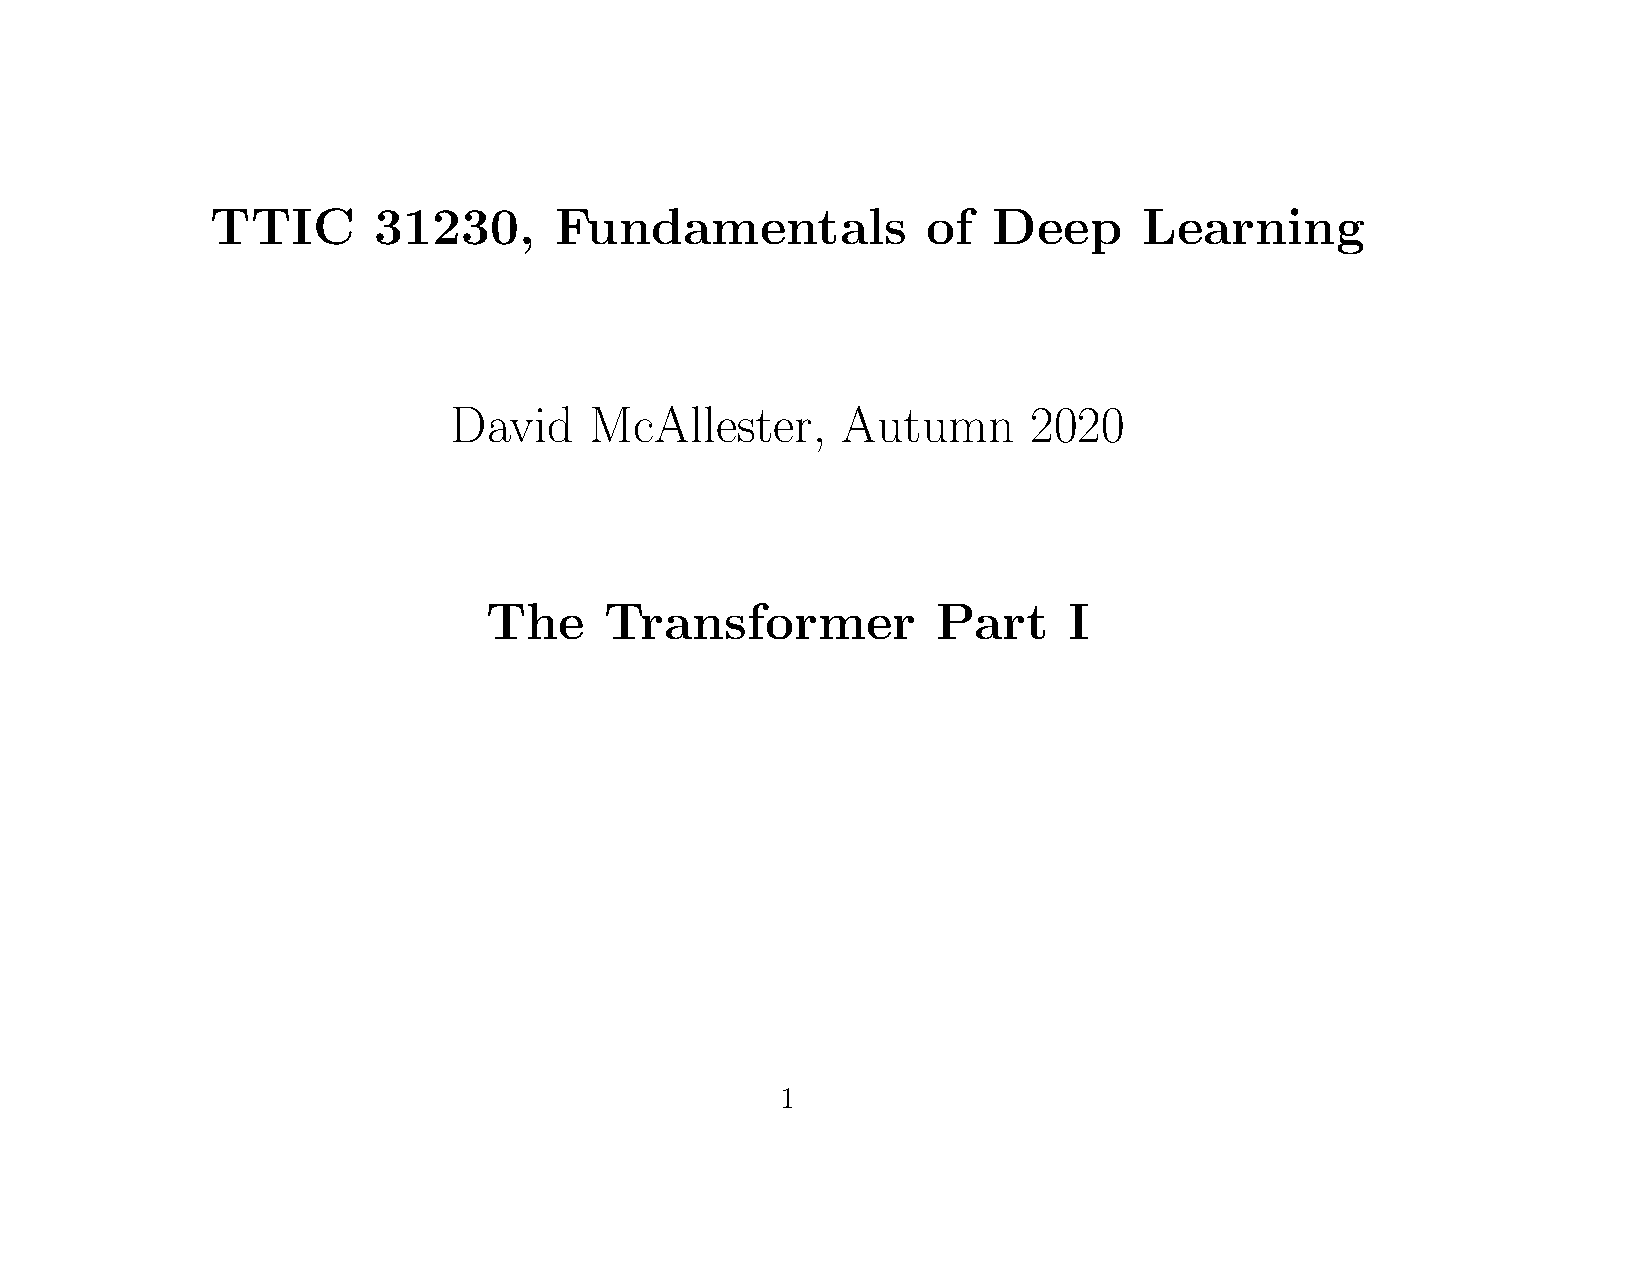
\includegraphics[height=4in]{\images/transformer}}

{\Large
\centerline{Jay Alammar's blog}
}

\slide{Layer Normalization}

The Transformer uses layer normalization rather than batch normalization to handle internal covariate shift.

\vfill
\begin{eqnarray*}
  \mu_\ell & = & \frac{1}{TJ} \sum_{t,j} \;L_\ell[t,j] \\
  \\
  \sigma_{\ell} & = & \sqrt{\frac{1}{TJ} \sum_{t,j}\;(L_\ell[t,j] - \mu_\ell)^2} \\
  \\
  \tilde{L}_{\ell+1}[t,j] & = & \mathrm{ReLU}\left(\frac{A_{\ell+1}[j]}{\sigma_\ell}(L_\ell[t,j] -\mu_\ell) + B_{\ell+1}[j]\right)
\end{eqnarray*}

\slide{Feed-Forward Layers}

The feed-forward layers apply a two-level multi-layer perceptron (MLP) to the vector at each time position independently.

\vfill

\begin{eqnarray*}
h_{\ell+1}[t,i] & = & \mathrm{ReLU}(W^{\mathrm{FF1}}_{\ell+1}[i,J]\;L_\ell[t,J] - B^{\mathrm{FF1}}_{\ell+1}[i]) \\
\\
L_{\ell+1}[t,j] & = & W^{\mathrm{FF2}}_{\ell+1}[j,I]\;h_{\ell+1}[t,I] - B^\mathrm{FF2}_{\ell+1}[j]
\end{eqnarray*}

\slide{The Transformer}

\centerline{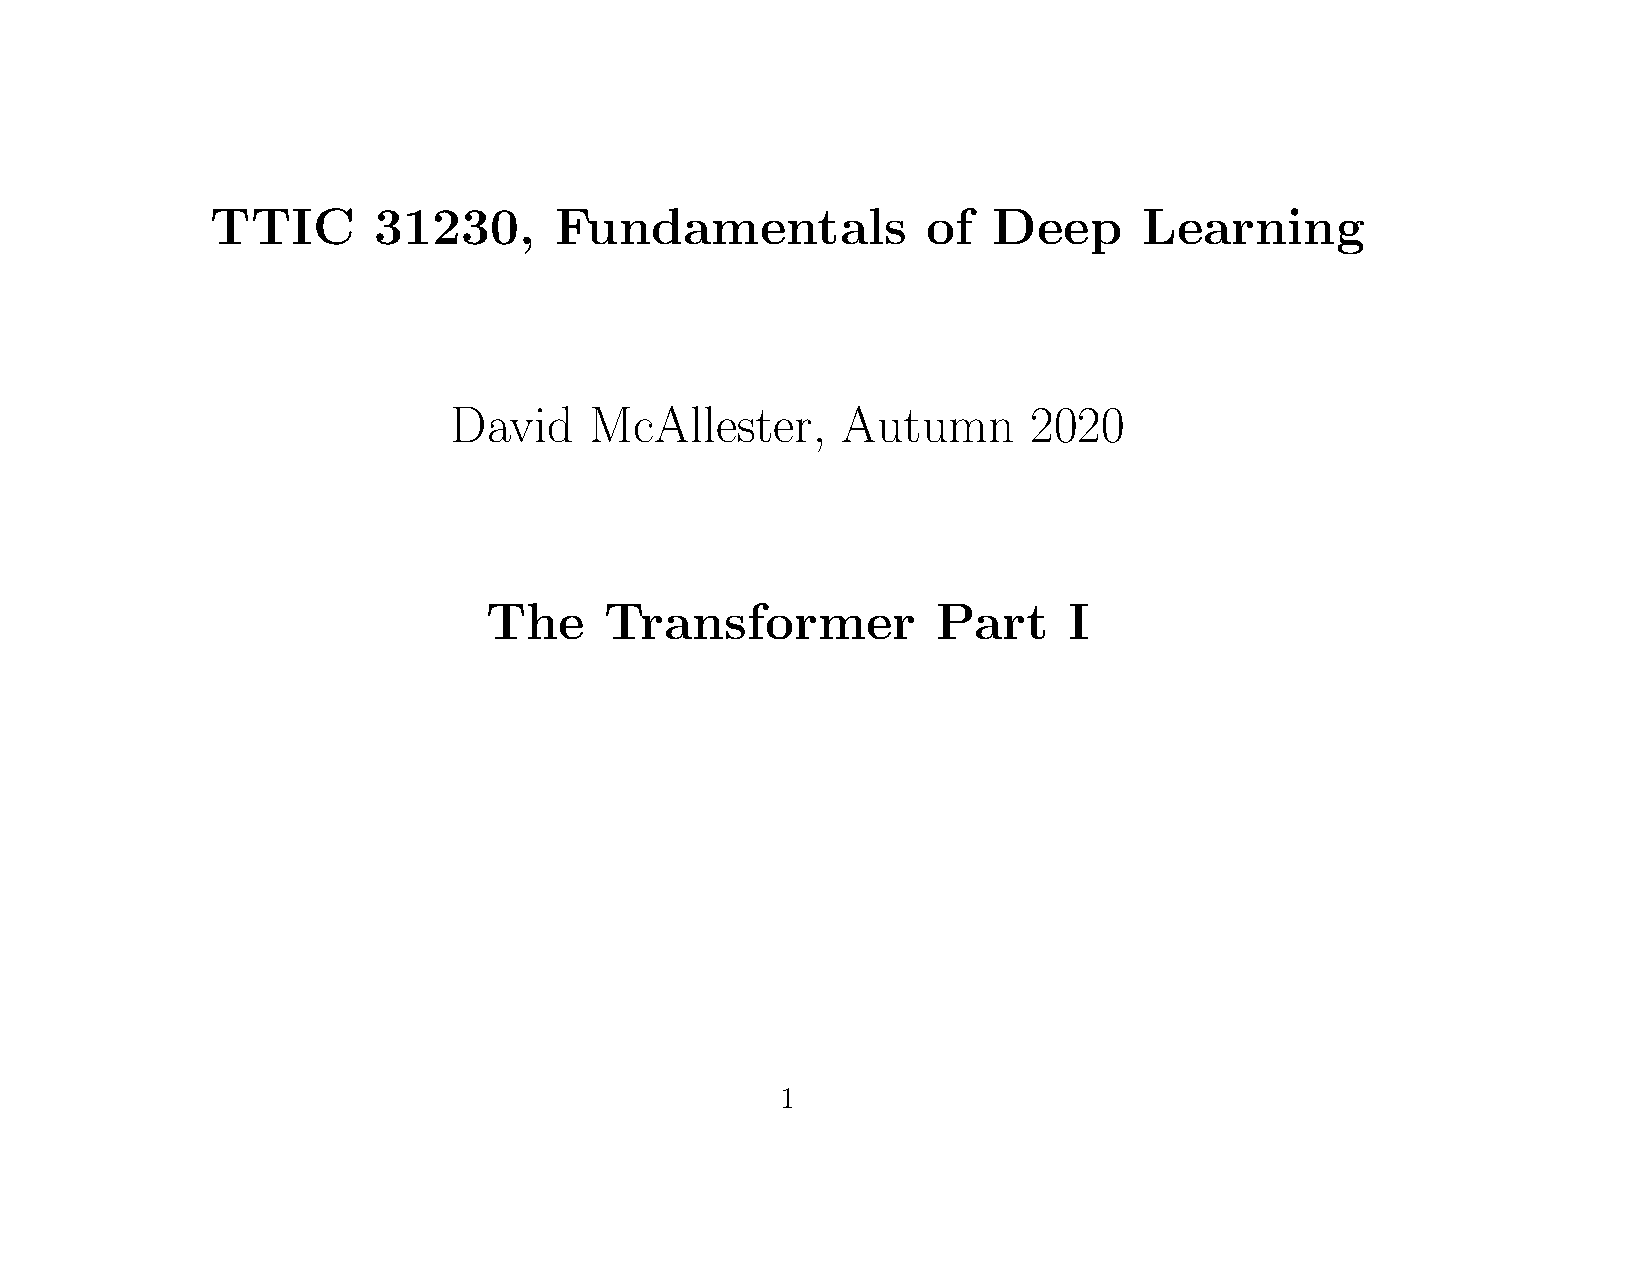
\includegraphics[height=4.5in]{\images/transformer}}

{\huge
\centerline{Jay Alammar's blog}
}

\slide{Encoding Positional Information}

At the input layer we concatenate the word embeddings with position embeddings.

\vfill
{\color{red} $$L_0[t,J] = e^W[w[t],I^W];e^T[t,I^P]$$}

\vfill
Note that without the position embeddings the model has no position information --- the input has to be treated as a bag of words.

\vfill
These days both word embedding and position embeddings are trained as model parameters.

\slide{Language Modeling}

To do language modeling we fix $\alpha[k,t_1,t_2] = 0$ for $t_2 > t_1$.

\vfill
We can then predict the word $w_t$ as without looking into the future with

\vfill
$$P(w_t|w_1,\ldots,w_{t-1}) = \softmax_{w_t}\;e[w_t,I]L_\mathrm{top}[t-1,I]$$

\vfill
where $L_\mathrm{top}$ is the top level hidden vector of the Transformer.

\slide{Machine Translation}

Translation is just a conditional language model.

\vfill
We take the input English sentence followed by a special token and then generate the output from the Transformer  language model.

\slide{Continuing from a Prompt}


GPT-2 from Open AI (1.5 billion parameters, June 2018)

\vfill
{\color{red} Continue from:}

\vfill
In a shocking finding, scientist discovered a herd of unicorns living in a remote, previously unexplored valley, in the Andes Mountains. Even more surprising to the researchers was the fact that the unicorns spoke perfect English.

\slide{The Predicted Continuation}

{\color{red} Continuation excerpted from a single response, the response selected from 10 tries.}

\bigskip

The scientist named the population, after their distinctive horn, Ovid’s Unicorn. These four-horned, silver-white unicorns were previously unknown to science.

Now, after almost two centuries, the mystery of what sparked this odd phenomenon is finally solved.

Dr. Jorge Pérez, an evolutionary biologist from the University of La Paz, and several companions, were exploring the Andes Mountains when ...
Pérez and his friends were astonished to see the unicorn herd. ...
While examining these bizarre creatures the scientists discovered that the creatures also spoke some fairly regular English. Pérez stated, “We can see, for example, that they have a common ‘language,’ something like a dialect or dialectic.”

Dr. Pérez believes that the unicorns may have originated in Argentina ... some believe that perhaps the creatures were created when a human and a unicorn met each other in a time before human civilization. ... However, Pérez also pointed out that it is likely that the only way of knowing for sure if unicorns are indeed the descendants of a lost alien race is through DNA. ...


\slide{Continuing from a Prompt}

GPT-3 from Open AI (175 billion parameters, July 2020, ArXiv 2005.14165)

\vfill
{\color{red} Continue from: Feeling unproductive? Maybe you should stop overthinking.}

\vfill
To In order to get something done, maybe we need to think less. Seems counter-intuitive, but I believe sometimes our thoughts can get in the way of the creative process. We can work better at times when we "tune out" the external world and focus on what's in front of us.

\vfill
I've been thinking about this lately, so I thought it would be good to write an article about it. 

\vfill
So what exactly does this mean? Well, for starters, let's start with some definitions.

\vfill
Definition \#1: Creative Thinking (CT) is the act of using your mind to come up with ideas that are not already present in reality or that have never existed before. It is a form of mental activity that involves the use of logic and reason.

\vfill
Definition \#2: Over-Thinking (OT) is the act of trying to come up with ideas that have already been thought through by someone else. OT usually results in ideas that are impractical, impossible, or even stupid.

\vfill
...

\slide{Few Shot Learning}

GPT-3 can be prompted with a sequence of German-to-English translation pairs ending in a German sentence without the English translation.

\vfill
GPT-3 continues with the English Translation of the given German.

\vfill
The translaion is not close to state of the art but still startling.

\vfill
Various other tasks can be done with few-shot examples in this way.  For example question answering, unscrambling words and three digit arithmetic.

\slide{Few Shot Learners}

A very recent paper (Sept. 15, 2020, ArXiv 2009.07118) has shown that the few-shot learning accomplishments of GPT-3 can be done with far fewer parameters.

\vfill
GPT-3 has 175 billion parameters.  The same few-shot performance can be achieved with 223 million parameters --- three orders of magnitude fewer.

\vfill
The new paper uses a method they call PET (Pattern Exploiting Training) involving ``distillation'' (student-teacher network-to-network training).

\slide{END}

}
\end{document}
